\section[Tracing]{Project Tracing}
% \frame{
%     \frametitle{Verfolgung von Projekten}
%     Tracing ist bestandteil der Dokumentation von Projekten. Prozessdoku.
%     OpenSource: Erfolgreiche OS-Projekte brauchen 4 Dinge: Projekt, Code, Dokumentation, Community.
%     Apache Way of Life.
%     H�ufigster Fehler: keine Doku.
%     Lehrbuchmodell: schreibt die Dokumentation schon vor.
%     Dokumentation ist aufwendig, deshalb automatisieren.
% }

% \frame{
%     \frametitle{Erfolgreiche Projekte}
%     Erfolgreiche Projekte brauchen 4 Dinge:
%     \begin{itemize}
%         \item das Projekt (bildet den Rahmen)
%         \item den Quellcode (klar!)
%         \item \alert<2>{ausf�hrliche Dokumentation (!!)}
%         \item eine Community / einen Kunden.
%     \end{itemize}
%     \vspace{0.5cm}
%     \invisible<1>{Zur Dokumentation geh�ren
%     \begin{itemize}
%         \item Beschreibung der Schnittstellen (API Dokumentation)
%         \item Ergebnisse der Unit-Tests inkl. Messung der Test�berdeckung
%         \item Erhebung und Visualisierung von Metriken
%         \item Produktdokumentation (Handb�cher, Online-Hilfe etc.)
%     \end{itemize}}
% }

% \frame{
%     \frametitle{Automatisierter Buildprozess}
%     Autmatisches Build gr��erer Projekte mit Ant und Make.
%     Nachteile:
%     \begin{itemize}
%         \item{Targets k�nnen nicht zwischen Projekten geteilt werden}
%         \item{Builddateien fast identisch}
%         \item{Kein Scripting m�glich (keine Loops/Conditionals)}
%         \item{Verwendung von 3rd-Party-Tools (z.B. javadoc) relativ umst�ndlich}
%         \item{Keine Aufl�sung von Library-Dependencies (Jar-H�lle)}
%     \end{itemize}
%     \vspace{0.5cm}
%     \large{\bf{L�sung:} Apache Maven}
% }


\frame{
    \frametitle{Project Tracing}
    \begin{block}{Ziel}
        Die Entwicklung bestimmter Projektparameter zu verfolgen.
        Wo steht mein Projekt jetzt in diesem Moment?
    \end{block}
    
    \begin{itemize}
        \item BWL-Sicht: Zeit, Resourcen, Kosten, Umfang
        \item Entwickler-Sicht: Qualit�t, Velocity, gute Dokumentation, Source-Metriken...
    \end{itemize}
}

\frame{
    \frametitle{Anatomie (eines Open-Source-Projekts)}
    \begin{columnsonlytextwidth}
    \begin{column}{5cm}
    \begin{itemize}
        \item Projekt ist ''nur'' die H�lle
        \item Eigentlicher Kern \begin{itemize}
            \item Code
            \item Dokumentation
            \item Community (Kunde)
        \end{itemize}
        \item Ohne diese 4 kann ein Projekt nicht erfolgreich sein.
    \end{itemize}
    \end{column}
    \begin{column}{5cm}
    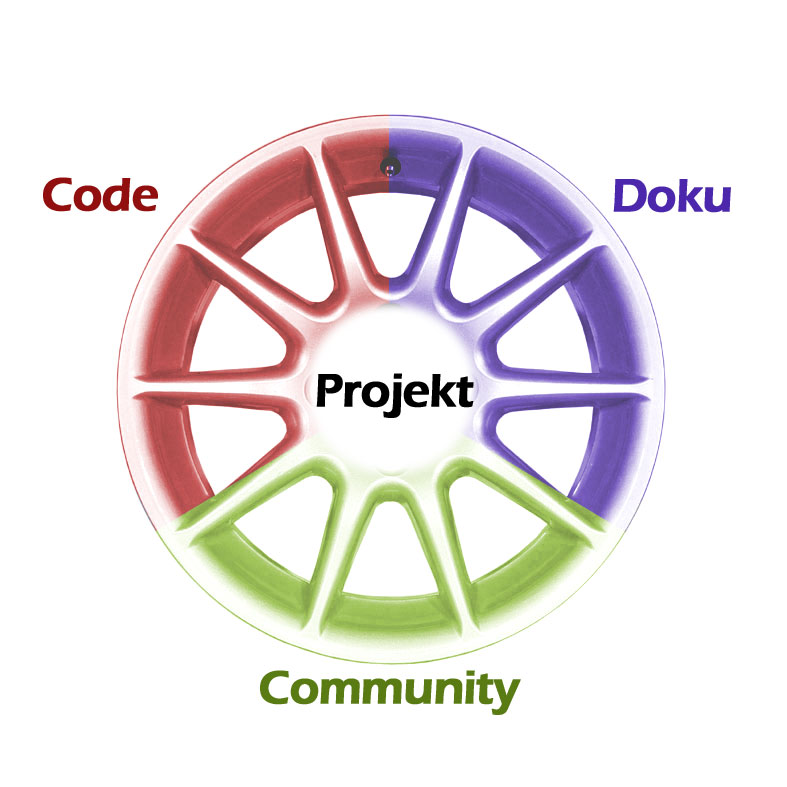
\includegraphics[width=5cm]{cdc}
    \end{column}
    \end{columnsonlytextwidth}
}

\frame{
    \frametitle{Project Tracing (in Open-Source-Projekten)}
    
    \begin{itemize}
        \item Einheitliche Dokumentation
        \item Architektur sichtbar machen
        \item Wer hat als letztes Was Wo gemacht? (Collective File Ownership)
        \item Qualit�tssicherung durch Source-Metriken
        \item Test�berdeckung
        \item �berblick �ber die verwendeten Bibliotheken
    \end{itemize}
    
    Das alles, und noch viel mehr: Automatisch im Buildprozess. Mit {\bf Apache Maven}.
}

